
%(BEGIN_QUESTION)
% Copyright 2006, Tony R. Kuphaldt, released under the Creative Commons Attribution License (v 1.0)
% This means you may do almost anything with this work of mine, so long as you give me proper credit

Anta at to lagringstanker av ulik størrelse begge inneholder gass ved samme lave trykk (mindre enn 1 PSI), uten noen væske i det hele tatt:

$$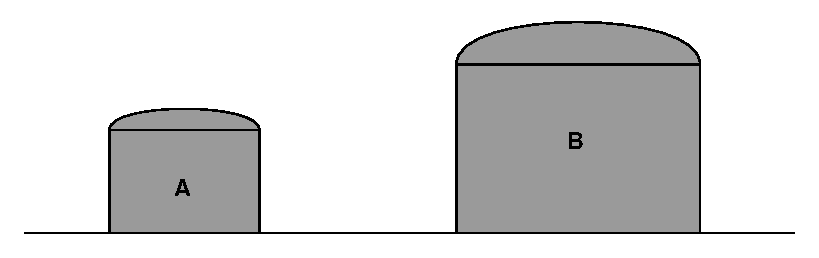
\includegraphics[width=15.5cm]{i00029x01.eps}$$

Bruk den ideelle gassloven ($PV = nRT$) til å bestemme hva som skjer med gasstrykket i disse to tankene når begge tankene varmes opp av sollys senere på dagen.  Anta at gasstrykkene var like da begge tanker var kalde (omgivelsestemperatur tidlig om morgenen), og at begge tanker er helt tette (ingen gass inn eller ut mens tankene varmes).  Velg det beste svaret som samsvarer med din prediksjon:

\vskip 10pt

\begin{itemize}
\item{} Begge tankenes trykk vil øke, og tank A sitt trykk vil øke mer enn tank B
\vskip 5pt
\item{} Begge tankenes trykk vil øke, og tank B sitt trykk vil øke mer enn tank A
\vskip 5pt
\item{} Begge tankenes trykk vil øke med samme beløp
\vskip 5pt
\item{} Tank A sitt trykk vil øke mens tank B sitt trykk vil synke
\vskip 5pt
\item{} Tank B sitt trykk vil øke mens tank A sitt trykk vil synke
\vskip 5pt
\item{} Begge tankenes trykk vil synke med samme beløp
\vskip 5pt
\item{} Begge tankenes trykk vil synke, og tank A sitt trykk vil synke mer enn tank B
\vskip 5pt
\item{} Begge tankenes trykk vil synke, og tank B sitt trykk vil synke mer enn tank A
\end{itemize}

\vfil

\underbar{file i00029}
\eject
%(END_QUESTION)





%(BEGIN_ANSWER)

Dette er et vurdert spørsmål -- ingen svar eller hint gis!

%(END_ANSWER)





%(BEGIN_NOTES)

Hvis begge tankene starter med samme temperatur og samme trykk, må vi konkludere med at mengden gassmolekyler i hver tank er proporsjonal med dens indre volum.  For enkel illustrasjon kan vi si at tank B har tre ganger så stort volum som tank A, og at tank B tilsvarende lagrer tre ganger så mange gassmolekyler som tank A.  I så fall vil en lik temperaturøkning i begge tankene gjøre at trykkene øker likt.  Derfor er det beste svaret, gitt lik temperaturøkning for begge, at: {\bf Begge tankenes trykk vil øke med samme beløp}

\vskip 10pt

Men . . . hvis vi antar at tankene varmes opp av sollys over en begrenset tidsperiode, er det mulig å konkludere med at tank A vil bli varmere enn tank B fordi forholdet mellom volum (masse) og overflateareal er mindre.  Når lineære dimensjoner på en tank øker, øker overflatearealet proporsjonalt med kvadratet av dimensjonene mens volumet øker proporsjonalt med kuben av dimensjonene.  Dette betyr at den minste av de to tankene (A) vil ha mer sol-absorberende overflate per lagret masse, og derfor vil varmes opp raskere enn den store tanken.  Hvis solen går ned før den større tanken har nådd temperaturen til den mindre tanken, er det beste svaret: {\bf Begge tankenes trykk vil øke, og tank A sitt trykk vil øke mer enn tank B}

%INDEX% Physics, static fluids: ideal gas law

%(END_NOTES)
